\documentclass{article}

\date{30 juin 2024}
\usepackage[nb-sem=28, auteurs={George Ober, Hugo Vangilluwen}]{../kholles}

\begin{document}
\maketitle

\begin{question_kholle}{Condition nécessaire de convergence de $\sum_{n \geqslant n_0} u_n$}
  Soit $u \in \K^{[ \! [ n_{0}, + \infty [ \![}$.
  Si la série $\sum_{n\geqslant n_{0}}u_{n}$ converge, alors la suite $u$ converge vers $0$.

  Supposons que la série converge. Notons $(S_{n})_{n\geqslant n_{0}}$ la suite des sommes partielles.
  $$\forall n \in [ \! [ n_{0}+1, +\infty [ \![, u_{n} = S_{n} - S_{n-1}$$
  Puisque $S$ converge, on en déduit que $u$ converge vers $0$.
\end{question_kholle}

\begin{question_kholle}[
    \begin{equation}
      \forall q \in \C, \
      \sum_{n \geqslant 0} q^n \text{ cv.}
      \iff |q| < 1
    \end{equation}
    Dans ce cas $\displaystyle \sum_{n=0}^{+\infty}q^{n}=\frac{1}{1-q}$ et $R_n = \frac{q^{n+1}}{1-q}$.
  ]{Condition nécessaire et suffisante de convergence de $\sum_{n\geqslant 0}q^{n}$ pour $q \in \C$ et calcul de la somme et du reste lorsqu'ils existent.}
  \begin{itemize}[label=$\star$]
    \item Si $\lvert q \rvert<1$
          $$\forall n \in \N, S_{n} = \sum_{k=0}^{n}q^{k} = \frac{1-q^{n+1}}{1-q}$$
          De plus, $\lvert q^{n+1} \rvert=\lvert q \rvert^{n+1}= \left\{ \begin{array}{ll}0 \text{ si }q=0\\ e^{(n+1)\ln \lvert q \rvert} \text{ si }q\neq 0\end{array}\right.$

          \begin{align*}
            \left\{ \begin{array}{ll}
                      0 \\
                      e^{(n+1)\ln \lvert q \rvert }
                    \end{array}\right. \xrightarrow[n\to \infty]{} \left\{ \begin{array}{ll}
                                                                             0 \\
                                                                             0
                                                                           \end{array}\right.
          \end{align*}

          Ainsi, $\sum_{n\geqslant 0}q^{n}$ converge et $\sum_{n=0}^{+\infty}q^{n}=\frac{1}{1-q}$
          $$S_{n} = \frac{1-q^{n+1}}{1-q} \implies R_{n} = S_{n} - \sum_{n=0}^{+\infty}q^{n}= \frac{q^{n+1}}{1-q}$$

    \item Si $\lvert q \rvert=1$

          $$\forall n \in \N, \lvert q \rvert ^{n} = 1^{n}=1 \xrightarrow[n \to \infty]{}1$$

          Ainsi, $\lvert q \rvert^{n}$ ne converge pas vers 0 donc $(q^{n})_{n\geqslant 0}$ ne converge pas vers 0, donc la série est grossièrement divergente.

    \item Si $\lvert q \rvert>1$
          $\lvert q \rvert^{n}=\exp(n \ln \lvert q \rvert) \xrightarrow[n\to +\infty]{} +\infty$
          Donc $(q^{n})_{n\geqslant 0}$ ne converge pas vers $0$. Donc la série est grossièrement divergente.
  \end{itemize}
\end{question_kholle}

\begin{question_kholle}[{Soit $\alpha \in \R$.
        \begin{equation}
          \text{La série } \sum_{n\geqslant 1} \frac{1}{n^{\alpha}} \text{ converge } \iff \alpha >1
        \end{equation}
      }]{Caractérisation de la convergence des séries de Riemann}
  \begin{itemize}[label=$\lozenge$]
    \item Supposons $\alpha < 0$ alors, $\frac{1}{n^{\alpha}}=n^{\lvert \alpha \rvert} \xrightarrow[n\to +\infty]{}+\infty$ donc la série est grossièrement divergente.
    \item Supposons $\alpha = 0$ alors $\frac{1}{n^{\alpha}}=1 \xrightarrow[n \to \infty]{} 1$ donc la série est grossièrement divergente.
    \item Supposons $\alpha > 0$
          Cherchons un équivalent de
          $$
            \frac{1}{(n+1)^{\beta}}-\frac{1}{n^{\beta}}
          $$
          en fonction de $\beta \in \R^{*}$

          \begin{align*}
            \frac{1}{(n+1)^{\beta}} - \frac{1}{n^{\beta}} & =
            \frac{1}{n^{\beta}}\left( \frac{1}{\left( 1+\frac{1}{n} \right)^{\beta}} - 1 \right)                                                                \\
                                                          & = \frac{1}{n^{\beta}}\left[ \left( 1+\frac{1}{n} \right)^{-\beta} - 1\right]                        \\
                                                          & \underset{ \overset {\infty} {} } {\sim} \frac{1}{n^{\beta}} \times \left( -\frac{\beta}{n} \right) \\
                                                          & \underset{ \overset {\infty} {} } {\sim} - \frac{\beta}{n^{\beta+1}}
          \end{align*}

          \begin{itemize}[label=$\star$]
            \item Pour $\alpha \in ]0, +\infty[ \setminus \left\{ 1 \right\}$
                        Appliquons le calcul ci-dessus pour $\beta \leftarrow \alpha -1$ (autorisé car $\alpha \neq 1\implies \alpha-1 \neq 0$)
                        $$\frac{1}{(n+1)^{\alpha-1}}-\frac{1}{n^{\alpha-1}} \underset{ \overset {\infty} {} } {\sim}
                          -\frac{\alpha-1}{n^{\alpha}}$$
                        De plus, $\left( -\frac{\alpha-1}{n^{\alpha}} \right)_{n\geqslant 1}$ est de signe constant donc, d'après le critère d'équivalence, $\sum_{n\geqslant 1} \frac{-(\alpha -1)}{n^{\alpha}}$ est de même nature que la série télescopique $\sum_{n\geqslant 1}(\frac{1}{(n+1)^{\alpha-1}}-\frac{1}{n^{\alpha-1}} )$. Or, la série télescopique est de même nature que $\left( \frac{1}{n^{\alpha-1}} \right)_{n\geqslant 1}$.

                        Donc par transitivité, puisque $\sum_{n\geqslant 1} \frac{1}{n^{\alpha}}$ est de même nature que $\sum_{n\geqslant 1} \frac{-(\alpha-1)}{n^{\alpha}}$, la série de Riemann est de même nature que $\left( \frac{1}{n^{\alpha-1}} \right)_{n\geqslant 1}$
                        Or, $\left( \frac{1}{n^{\alpha-1}} \right)_{n\geqslant 1}$ converge pour $\alpha>1$ et diverge pour $\alpha \in ]0, 1[$.

            \item Si $\alpha = 1$
                  Appliquons la comparaison série intégrale pour $f \leftarrow (x \mapsto \frac{1}{x}) \left\{ \begin{array}{ll} \in \mathcal{C}^{0}([1, +\infty[, \R)\\ \text{décroissante sur }[1, +\infty[ \end{array}\right.$

                  $$\forall n \in \N^{*}, \int_{1}^{n+1}  \frac{\mathrm{d}u}{u} \leqslant  \sum_{k=1}^{n} \frac{1}{k}$$
                  Ainsi,
                  $$\forall n \in \N^{*}, \underbrace{ \ln(n+1) }_{ \xrightarrow[n \to +\infty]{} +\infty } \leqslant \sum_{k=1}^{n} \frac{1}{k}$$
                  Donc la série diverge.
          \end{itemize}
  \end{itemize}
\end{question_kholle}

\begin{question_kholle}[
  Soit $n_0 \in \N$.
  Soit $f:[n_0, +\infty[ \to \R$ une fonction continue et décroissante. Nous avons l'encadrement suivant :
      \begin{equation}
        \int_{n_{0}}^{n+1} f(t) \, \mathrm dt \leqslant
        \sum_{k=n_{0}}^{n} f(k)
        \leqslant f(n_{0})+ \int_{n_{0}}^{n} f(t) \, \mathrm dt
      \end{equation}
    ]{Comparaison série-intégrale}
    Soit $k \in [ \! [ n_{0}, +\infty [\![$ fixé quelconque.

  \begin{align*}
    \forall t \in [k, k+1], \ f(k+1)    & \leqslant f(t) \leqslant f(k)                                                            \\
    \int_{k}^{k+1} f(k+1) \, \mathrm dt & \leqslant \int_{k}^{k+1} f(t) \, \mathrm dt \leqslant \int_{k}^{k+1}  f(k) \, \mathrm dt \\
    f(k+1)                              & \leqslant \int_{k}^{k+1} f(t) \, \mathrm dt \leqslant f(k)
  \end{align*}

  Ainsi

  \begin{align*}
    \sum_{k=n_{0}}^{n}\int_{k}^{k+1}f(t)  \, \mathrm dt & \leqslant \sum_{k=n_{0}}^{n}f(t) \\
    \int_{n_{0}}^{n+1} f(t) \, \mathrm dt               & \leqslant \sum_{k=n_{0}}^{n}f(k)
  \end{align*}


  De même,

  \begin{align*}
    \forall k \in [ \! [ n_{0}+1 , \ +\infty[ \![, f(k) & \leqslant\int_{k-1}^{k} f(t) \, \mathrm dt                      \\
    \sum_{k=n_{0}+1}^{n}f(k)                            & \leqslant \sum_{k=n_{0}+1}^{n}\int_{k-1}^{k} f(t) \, \mathrm dt \\
    \sum_{k=n_{0}}^{n} f(k)                             & \leqslant f(n_{0})+ \int_{n_{0}}^{n} f(t) \, \mathrm dt
  \end{align*}

  D'où l'encadrement.
\end{question_kholle}

\begin{question_kholle}[{Soit $n_{0} \in \N$ et $f:[n_{0}, +\infty[ \to \R$ une fonction continue, décroissante et minorée par $m \in \R$.
  Alors la série de terme général
  $$\left( f(n)- \int_{n}^{n+1} f(u) \, \mathrm du  \right)_{n\geqslant n_{0}}$$
  est à termes positifs ou nuls et converge.
  }]{Pour $f$ continue sur $[n_0, +\infty[$, décroissante et minorée, $\displaystyle\sum_{n\geqslant n_{0}}\left( f(n)- \int_{n}^{n+1} f(u) \, \mathrm du  \right)$ converge. Application au DA en $o(1)$ de la somme partielle de la série harmonique}

  Montrons que la suite $(S_{n})_{n\geqslant n_{0}}$ est majorée, et que la suite est à termes $\geqslant 0$
  
  La décroissance de $f$ donne l'encadrement suivant

  $$\forall n \in [ \! [ n_{0} , +\infty[\![,  f(n) - \int_{n}^{n+1} f(t) \, \mathrm dt \geqslant 0$$

  La comparaison série intégrale s'applique donc à $f$ qui est décroissante et continue et donne

  \begin{align*}
    \forall n \in [ \! [ n_{0}, +\infty [ \![ f(n+1)\leqslant \int_{n}^{n+1} f(t) \, \mathrm dt \leqslant f(n) & \implies -f(n+1) \geqslant -\int_{n}^{n+1} f(t) \, \mathrm dt                          \\
                                                                                                               & \implies f(n) - f(n+1) \geqslant f(n) - \int_{ n}^{n+1} f(t) \, \mathrm dt \geqslant 0
  \end{align*}

  En sommant sur $k \in [ \! [ n_{0}, n ] \!]$

  $$\sum_{k=n_{0}}^{n} (f(k) - f(k+1)) \geqslant  \sum_{k=n_{0}}^{n}\left( f(k) - \int_{k}^{k+1} f(t) \, \mathrm dt  \right) = S_{n}$$

  En reconnaissant un phénomène télescopique

  $$S_{n} \leqslant f(n_{0})-f(n+1)\leqslant f(n_{0})- m $$

  Donc $(S_{n})_{n\geqslant n_{0}}$ est croissante et majorée, elle converge.
  \\

  \begin{figure}[H]
    \centering
    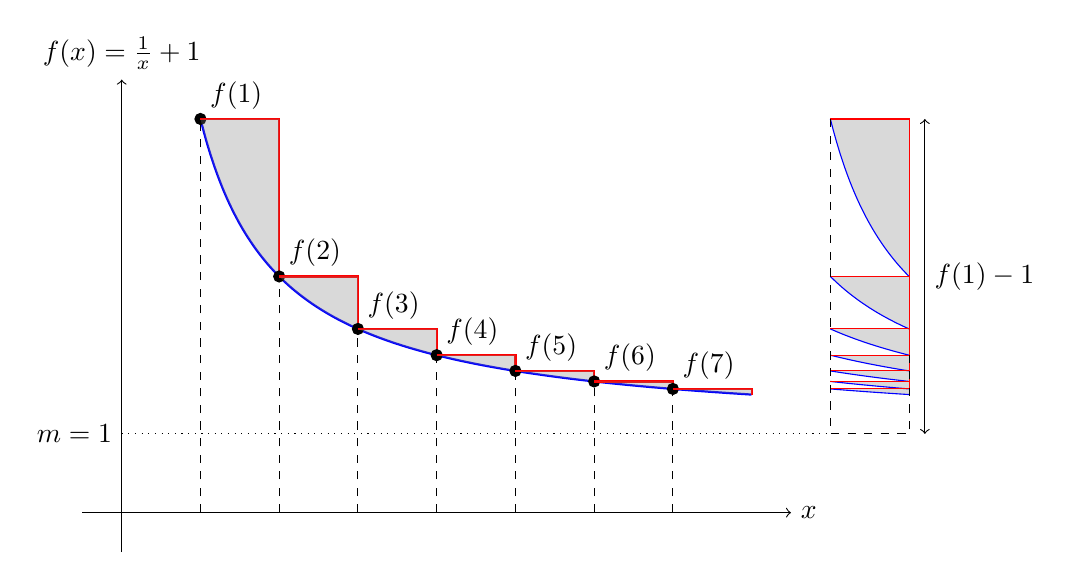
\begin{tikzpicture}

      \draw[->] (-0.5,0) -- (8.5,0) node[right] {$x$}; % x-axis
      \draw[->] (0,-0.5) -- (0,5.5) node[above] {$f(x) = \frac{1}{x} + 1$}; % y-axis
      
      \draw[domain=1:8,samples=100,smooth,thick,blue] plot (\x, {1/\x*4 + 1}) node[right] {};
      
      \foreach \n in {1,2,...,7} {
          
          \draw[dashed] (\n, 0) -- (\n, {4/\n + 1}); 
          \filldraw (\n, {4/\n + 1}) circle (2pt) node[above right] {$f(\n)$};
          
          
          \draw[red, thick] (\n, {4/\n + 1}) -- (\n+1, {4/\n + 1}) -- (\n+1, {1 + 4/(\n + 1)});
          
          \fill[gray, opacity=0.3] 
              plot[domain=\n:\n+1, samples=50] (\x, {1 + 4/\x}) -- 
              (\n+1, {1 + 4/\n}) -- (\n, {1 + 4/\n}) -- cycle;
          
          \fill[gray, opacity=0.3] 
              plot[domain=\n:\n+1, samples=50] (\x - \n + 9, {1+ 4/\x}) -- 
              (10, {1 + 4/\n}) -- (9, {1+ 4/\n}) -- cycle;
      
          \draw[blue] plot[domain = \n:\n+1, samples = 50] (\x - \n + 9, {1 + 4/\x});
          \draw[red] (9, {1 + 4/\n}) -- (10, {1 + 4/\n}) -- (10, {1 + 4/(\n+1)});
      }
      
      \draw[dashed] (9, 5) -- (9, 1) -- (10, 1) -- (10, 2);
      \draw[dotted] (0, 1) node[left] {$m = 1$} -- (9, 1);
      
      \draw[<->] (10.2, 1) -- (10.2, 5) node[pos=0.5, right] {$f(1) - 1$};
      
      \end{tikzpicture}
      \caption{Une visualisation graphique de la bornitude de $(S_n)_{n \geqslant n_0}$ pour le cas particulier de $f \leftarrow (x \mapsto \nicefrac 1 x + 1), m \leftarrow 1, n_0 \leftarrow 1$. On interprète chaque terme de la somme comme l'aire du rectangle à laquelle on retranche l'aire sous la courbe : cela correspond à l'aire grise, qui peut être aisément installée dans un rectangle d'aire $f(1) - 1 = f(n_0) - m$.}
  \end{figure}

  \textit{Application au DA en $o(1)$ de la somme partielle de la série harmonique.}
  Appliquons ce qui précède pour $f = x \mapsto \nicefrac{1}{x}$ et $n_0 = 1$. $f$ est bien continue, décroissante et minorée (par 0). sur $[1; + \infty[$.
  Donc $\displaystyle \sum_{ n \geqslant 1} \left( \frac{1}{n} - \int_{n}^{n+1} \frac{\mathrm du}{u} \right)$ converge.

  Notons $\gamma$ sa somme. Ainsi $\displaystyle \sum_{k=1}^{n} \left( \frac{1}{k} - \int_{k}^{k+1} \frac{\mathrm du}{u} \right) \underset{n \to +\infty}{=} \gamma + o(1)$.

  Remarquons que, pour tout $n \in \N$,
  $\displaystyle \sum_{k=1}^{n} \left( \frac{1}{k} - \int_{k}^{k+1} \frac{\mathrm du}{u} \right)
    = H_n - \sum_{k=1}^{n} \left( \ln(k+1) - \ln(k) \right)
    = H_n - \ln(n+1) + \ln 1
    = H_n - \ln(n+1)$.

  Donc $H_n \underset{n \to +\infty}{=} \ln(n+1) + \gamma + o(1) = \ln n + \ln \left( 1 + \nicefrac{1}{n} \right) + \gamma + o(1)$.
  \begin{equation*}
    H_n \underset{n \to +\infty}{=} \ln n + \gamma + o(1)
  \end{equation*}
  La constante $\gamma$ est appelé la constante d'Euler-Mascheroni et vaut environ $0,5772156649$.
\end{question_kholle}

\begin{question_kholle}[{Soit $(a_{n})_{n\geqslant n_{0}} \in \R^{[ \! [ n_{0}, +\infty [ \![}$ une suite réelle.
  Si
  $$
    \left\{ \begin{array}{ll}
      \forall n \in [ \! [ n_{0}, +\infty [\![, a_{n} \geqslant 0 \\
      (a_{n})_{n\geqslant n_{0}} \text{ est décroissante}         \\
      \lim_{ n \to \infty } a_{n}=0
    \end{array}\right.
  $$
  alors $\sum_{n\geqslant n_{0}}(-1)^{n}a_{n}$}]{Théorème des séries alternées}

  \begin{itemize}[label=$\lozenge$]
    \item Traitons le cas $n_{0}\equiv 0 [2]$ il existe $p_{0} \in \N: n_{0}=2p_{0}$
          \begin{itemize}[label=$\star$]
            \item  Les suites $(S_{2p})_{p\geqslant p_{0}}$ et $(S_{2p+1})_{p\geqslant p_{0}}$ sont adjacentes:

                  \begin{align*}
                    \forall p \in [ \! [ p_{0}, +\infty[ \![, S_{2(p+1)} - S_{2p} & = S_{2p+2}- S_{2p}                                                        \\
                                                                                  & = \sum_{k=2p_{0}}^{2p+2}(-1)^{k}a_{k} + \sum_{k=2p_{0}}^{2p}(-1)^{k}a_{k} \\
                                                                                  & = -a_{2p+1}+a_{2p+2} \leqslant 0 \text{ car }a\downarrow
                  \end{align*}

                  \begin{align*}
                    S_{2(p+1)+1} - S_{2p+1} & = S_{2p+3} - S_{2p+1} = (-1)^{2p+2}a_{2p+2}+(-1)^{2p+3}a_{2p+3} = a_{2p+2}- a_{2p+3} \geqslant 0 \text{ car }a\downarrow
                  \end{align*}


                  Donc $(S_{2p})$ est décroissante et $(S_{2p+1})$ est croissante.
                  De plus
                  $$
                    S_{2p+1} - S_{2p} = (-1)^{2p+2}a_{2p+1} = \underbrace{ -a_{2p+1} }_{ \xrightarrow[p \to \infty]{} 0 } \leqslant 0 \text{ car a positive}
                  $$
                  Ainsi $(S_{2p})_{p\geqslant p_{0}}$ et $(S_{2p+1})_{p\geqslant p_{0}}$ sont adjacentes.
            \item Donc d'après le théorème des suites adjacentes, $(S_{2p})$ et $(S_{2p+1})$ convergent vers une même limite $\ell$, si bien que $(S_{n})$ converge vers $\ell$.

            \item De plus, les suites $(S_{2p})_{p\geqslant p_{0}}$ et $(S_{2p+1})_{p\geqslant p_{0}}$ étant adjacentes, pour $n \geqslant n_{0}$ posons $R_{n} = \ell -S_{n}$
                  \begin{itemize}
                    \item Si $n \equiv 0 [2]$, $\exists p \in [ \! [ p_{0}, +\infty [ \![:n=2p$ donc, puisque $(S_{2p})$ est décroissante et $(S_{2p+1})$ est croissante, on a
                          $$
                            S_{2p+1}\leqslant \ell \leqslant S_{2p} \implies S_{2p+1} - S_{2p} \leqslant \ell - S_{2p} \leqslant 0 \implies \lvert R_{2p} \rvert = \lvert \ell - S_{2p} \rvert \leqslant a_{2p+1}
                          $$

                    \item Si $n \equiv 1 [2]$ $\exists p \in [ \! [ p_{0}, +\infty [ \![:n=2p+1$
                          $$
                            S_{2p+1} \leqslant \ell \leqslant S_{2p+2} \implies 0 \leqslant \ell - S_{2p+1} \leqslant S_{2p+2} - S_{2p+1} = (-1)^{2p+2}a_{2p+2}= a_{2p+2}
                          $$
                          donc $\lvert R_{2p+1} \rvert = \lvert \ell-S_{2p+1} \rvert \leqslant a_{2p+2}$
                  \end{itemize}
          \end{itemize}
          Bonus, par croissance de $(S_{2p+1})$ qui converge vers $\ell$, $S_{2p+1} \leqslant \ell$  donc $a_{2p_{0}}-a_{2p_{0} +1}\leqslant\ell$
          Donc $\ell \geqslant 0$ qui est bien le signe du premier terme de la série $(-1)^{n_{0}}a_{n_{0}}$ car $n_{0}\equiv 0[2]$.

    \item Le cas $n_0 \equiv 1 [2]$ se traite de la même manière
  \end{itemize}
\end{question_kholle}

\begin{question_kholle}[{Soit $u \in \K^{[ \! [ n_{0}, +\infty [ \![}$
  Si la série $\sum_{n\geqslant n_{0}}u_{n}$ est absolument convergente, alors la série $\sum_{n\geqslant n_{0}}u_{n}$ est convergente.}]{L'absolue convergence implique la convergence}



  \begin{itemize}[label=$\lozenge$]
    \item Supposons que $u$ est le terme général réel d'une série absolument convergente.
          Posons, pour tout $n \in [ \! [ n_{0}, +\infty [ \![$, $u_{n}^{+}= \max(u_{n}, 0)$ et $u_{n}^{-}=- \min (u_{n}, 0)$
          Avec ces notations, $u_{n}^{+}- u_{n}^{-} = u_{n}$ et $u_{n}^{+}+u_{n}^{-} = \lvert u_{n} \rvert$.
          $$
            \forall n \in [ \! [ n_{0}, +\infty [ \![, u_{n}^{+}\geqslant 0 \text{ et } u_{n}^{-}\geqslant 0
          $$

          $$
            \left. \begin{array}{ll}
              \forall n \geqslant n_{0}, 0\leqslant u_{n}^{+} \leqslant \lvert u_{n} \rvert = u_{n}^{+}+ u_{n}^{-}           \\
              \sum_{n\geqslant n_{0}} u_{n} \text{ est ACV} \implies \sum_{n\geqslant n_{0}} \lvert u_{n} \rvert  \text{ CV} \\
              \forall n \geqslant n_{0}, u_{n}^{+}\geqslant 0 \text{ et } \lvert u_{n} \rvert \geqslant 0
            \end{array}\right\}\implies \sum_{n\geqslant n_{0}}u_{n} ^{+}\text{ converge}
          $$

          On montre de même que $\sum_{n\geqslant n_{0}}u_{n}^{-}$ converge, donc, par structure vectorielle de l'ensemble des termes généraux de suites convergentes, $\sum_{ n\geqslant n_{0}}(u_{n}^{+} - u_{n}^{-})= \sum_{n\geqslant n_{0}}u_{n}$ converge
          \begin{figure}[H]
            \centering
            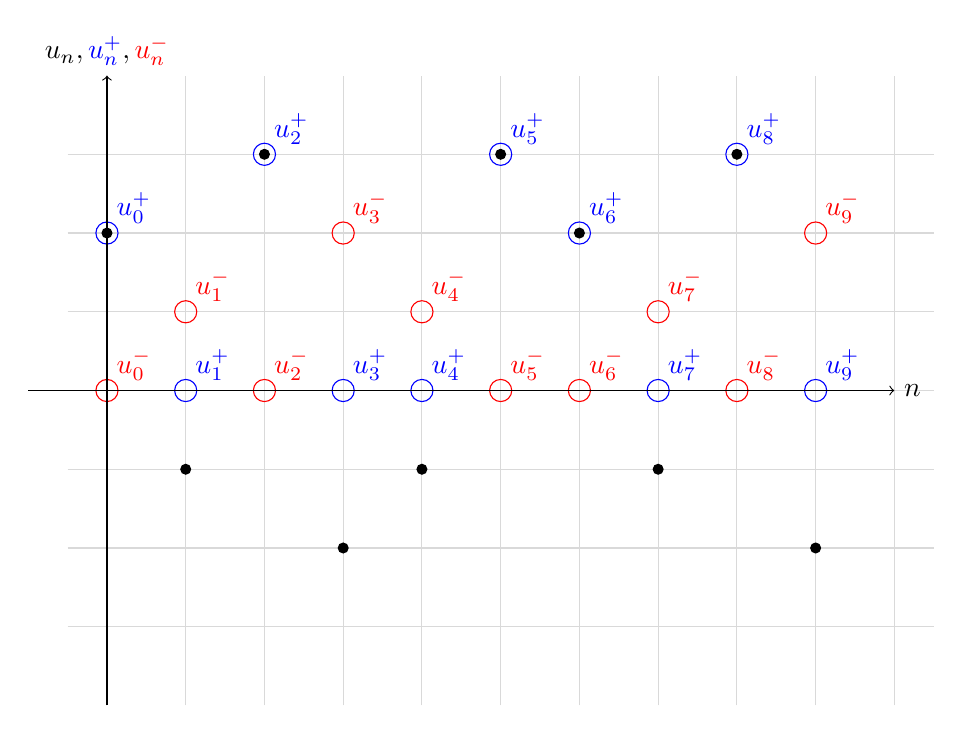
\begin{tikzpicture}
              \def\numbers{{2.5, -1.8, 3.2, -2.5, -1.5, 3, 2.8, -1.2, 3.5, -2}}
          
          
              \foreach \y in {-3,-2,-1,0,1,2,3}
              \draw[gray!30] (-0.5,\y) -- (10.5,\y);
              \foreach \x in {1,2,3,4,5,6,7,8,9,10}
              \draw[gray!30] (\x,-4) -- (\x,4);
          
              \foreach \i in {0,1,2,3,4,5,6,7,8,9} {
                  \pgfmathtruncatemacro{\number}{\numbers[\i]}
          
                  \fill[black] (\i, \number) circle (2pt);
          
                  \ifnum\number>0
                      \draw[blue] (\i, \number) circle (4pt) node[above right] {$u_\i^+$};
                      \draw[red] (\i, 0) circle (4pt) node[above right] {$u_\i^-$};
                  \else        
                      \draw[red] (\i, -\number) circle (4pt) node[above right] {$u_\i^-$};
                      \draw[blue] (\i, 0) circle (4pt) node[above right] {$u_\i^+$};
                  \fi
              }
              
          
              \draw[->] (-1, 0) -- (10, 0) node[right] {$n$};
              \draw[->] (0, -4) -- (0, 4) node[above] {$u_n, {\color{blue} u_n^+}, {\color{red} u_n^-}$};
              
            \end{tikzpicture}
            \caption{Décomposition de la suite $u$ en $u^+$ et $u^-$, les "partie positive" et "partie négative". Graphiquement, on retrouve $u_n^+ + u_n^- = |u_n|$ et $u_n^+ - u_n^- = u_n$}
          \end{figure}
    \item Cas d'une série complexe,

          Posons, $\forall n\geqslant n_{0}, x_{n} = \mathrm{Re}(u_{n})$ et $y_{n} = \mathrm{Im}(u_{n})$
          Alors,
          $$
            \left. \begin{array}{ll}
              \forall n \geqslant n_{0}, \lvert x_{n} \rvert \leqslant \lvert \mathrm{Re}(u_{n}) \rvert \leqslant \lvert u_{n} \rvert \\
              \forall n\geqslant n_{0}, \lvert  x_{n} \rvert \geqslant 0 \text{ et } \lvert u_{n} \rvert \geqslant 0                  \\
              \sum_{n\geqslant n_{0}}u_{n} \text{ ACV } \implies \sum_{n\geqslant n_{0}}\lvert u_{n} \rvert \text{ CV }
            \end{array}\right\}\implies \sum_{n\geqslant n_{0}}\lvert x_{n} \rvert \text{ converge}
          $$
          Donc d'après le cas réel, $\sum_{n\geqslant n_{0}} x_{n}$ converge
          On montre de même que $\sum_{n\geqslant n_{0}}y_{n}$ converge
          Donc, par structure vectorielle, $\sum_{n\geqslant n_{0}}(x_{n}+ iy_{n})$ converge.
          Donc $u_{n}$ est le terme général d'une série convergente.
        \end{itemize}
        
\end{question_kholle}

\begin{question_kholle}
  {Décomposition d'une permutation en produit de cycles à supports disjoints puis en produit de transposition et calcul de son ordre}
  Prenons pour illustrer la décomposition
  \begin{equation*}
    \sigma = \begin{pmatrix}
      1 & \mapsto & 6 \\
      2 & \mapsto & 4 \\
      3 & \mapsto & 3 \\
      4 & \mapsto & 2 \\
      5 & \mapsto & 1 \\
      6 & \mapsto & 5 \\
    \end{pmatrix}
    \in \mathcal{S}_6
  \end{equation*}

  Il faut réaliser un "graphe des images". Chaque sommet est un nombre de $\lient 1; 6 \rient$ et pointe vers son image.

  \begin{figure}[H]
    \centering
    \begin{tikzpicture}[
        node distance={15mm},
        thick,
        edge/.style = {draw, circle},
        arrow/.style = {thick,
            arrows={
                - Stealth[length=8pt,open,bend,width=3mm]
              }
          }
      ]

      \node (1) {1};
      % 1/sqrt(3) = 0.58
      \node (5) [below right=1cm and 0.58cm of 1] {5};
      \node (6) [below left=1cm and 0.58cm of 1] {6};
      \node (2) [right=2cm of 1] {2};
      \node (4) [below=1cm of 2] {4};
      \node (3) [right=1cm of 2] {3};

      \draw[arrow] (1) edge [bend right=30] (6);
      \draw[arrow] (6) edge [bend right=30] (5);
      \draw[arrow] (5) edge [bend right=30] (1);

      \draw[arrow] (2) edge [bend right=30] (4);
      \draw[arrow] (4) edge [bend right=30] (2);

      %			\draw[arrow] (3) edge [bend right=45] (3);
      \draw [arrow] (3.200) arc (90:400:3mm) (3);
    \end{tikzpicture}
  \end{figure}

  Nous pouvons voir que $\sigma = (1, 6, 5) \circ (2, 4)$.
  De plus, $(1, 6, 5) = (1, 6) \circ (6, 5) \circ (5, 1)$.
  Donc $\sigma = (1, 6) \circ (6, 5) \circ (5, 1) \circ (2, 4)$.

  L'ordre d'une permutation est définit par $p(\sigma) = \min \{ n \in \N^* \;|\; \sigma^n = Id \}$. $p(\sigma)$ est aussi le PPCM des ordres des permutations de sa décomposition en produit de cycles à supports disjoints. Ici, $p(\sigma) = 2 \vee 3 = 6$.
\end{question_kholle}
\end{document}
